\documentclass[lettersize,journal]{IEEEtran}
\usepackage{amsmath,amsfonts}
\usepackage{algorithmic}
\usepackage{algorithm}
\usepackage{array}
\usepackage[caption=false,font=normalsize,labelfont=sf,textfont=sf]{subfig}
\usepackage{textcomp}
\usepackage{stfloats}
\usepackage{url}
\usepackage{verbatim}
\usepackage{graphicx}
\usepackage{cite}
\usepackage{booktabs}
\usepackage{multirow}
\hyphenation{op-tical net-works semi-conduc-tor IEEE-Xplore}
% updated with editorial comments 8/9/2021

\begin{document}

\title{A Sample Article Using IEEEtran.cls\\ for IEEE Journals and Transactions}

\author{IEEE Publication Technology,~\IEEEmembership{Staff,~IEEE,}
        % <-this % stops a space
\thanks{This paper was produced by the IEEE Publication Technology Group. They are in Piscataway, NJ.}% <-this % stops a space
\thanks{Manuscript received April 19, 2021; revised August 16, 2021.}}

% The paper headers
\markboth{Journal of \LaTeX\ Class Files,~Vol.~14, No.~8, August~2021}%
{Shell \MakeLowercase{\textit{et al.}}: A Sample Article Using IEEEtran.cls for IEEE Journals}

\IEEEpubid{0000--0000/00\$00.00~\copyright~2021 IEEE}
% Remember, if you use this you must call \IEEEpubidadjcol in the second
% column for its text to clear the IEEEpubid mark.

\maketitle

\begin{abstract}
This document describes the most common article elements and how to use the IEEEtran class with \LaTeX \ to produce files that are suitable for submission to the IEEE.  IEEEtran can produce conference, journal, and technical note (correspondence) papers with a suitable choice of class options. 
\end{abstract}

\begin{IEEEkeywords}
Article submission, IEEE, IEEEtran, journal, \LaTeX, paper, template, typesetting.
\end{IEEEkeywords}

\section{Introduction}
\IEEEPARstart{T}{his} file is intended to serve as a ``sample article file''


\section{Related work}
\subsection{Hyperbola recognition task}
\begin{figure}[]
    \centering
    \subfloat[]{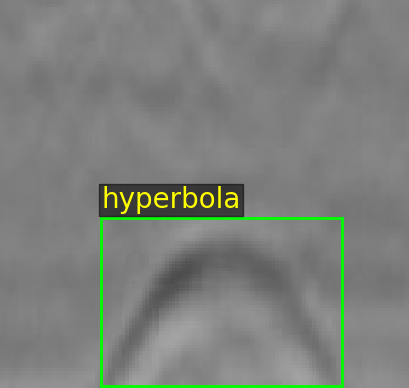
\includegraphics[width=0.42\linewidth]{shuangquxiansample1.png}}
    \subfloat[]{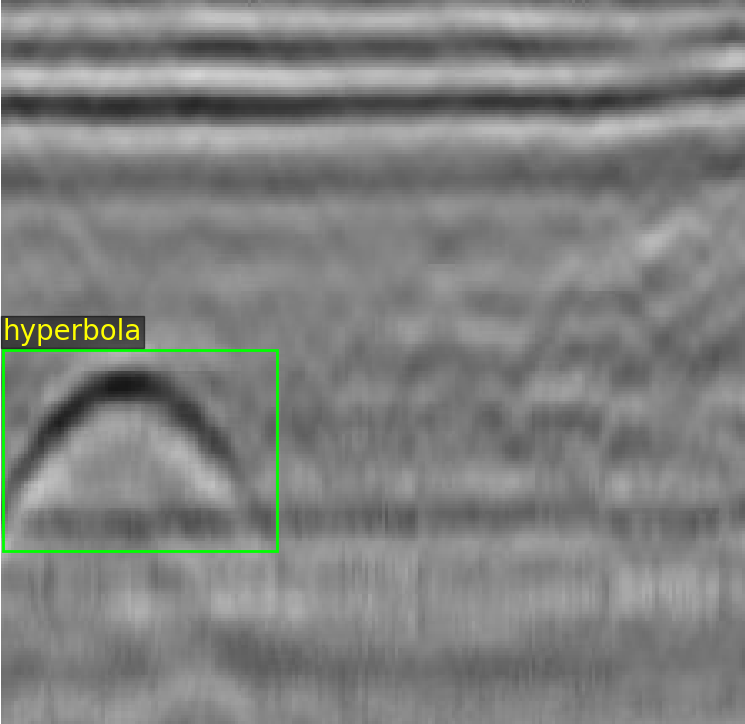
\includegraphics[width=0.41\linewidth]{shuangquxiansample2.png}}
    \caption{Hyperbola samples.}
    \label{fig:shaungquxiansamples}
\end{figure}


\subsection{Labelling tools}





\section{Proposed method}
\subsection{Hyperbola annotation tool}
%我们设计了一个 双曲线带状目标的可视化标注工具。该工具的使用界面如图所示。
%首先，选择图片的文件夹，然后会自动加载其中的图片
%然后下方左侧会显示原图，右侧会显示标注后的图片。
%在左图单击的点为双曲线的顶点位置，右侧可以调节各个参数。
%我们设定了5个参数。分别是双曲线顶点的横纵坐标，双曲线的宽度，曲率和带状厚度。
%点 Add as New Annotation 把当前参数作为一个新标注加入当前图片，并且可以在同一个图中添加多个标注。
%我们的标注通过json格式保存
%格式为{
  % "001.jpg": [
  %   {
  %     "label": "hyperbola",
  %     "x_vertex": 148.16,
  %     "y_vertex": 194.24,
  %     "width": 60.0,
  %     "height": 30.0,
  %     "thickness": 12.0
  %   }
  % ],
  % }
%001.jpg是图片的名字，其余是参数和对应的值
We designed a visual annotation tool for hyperbolic ribbon-shaped targets, whose user interface is illustrated in the Fig.~\ref{fig:tool}.
First, the user selects an image folder, and the tool automatically loads all images within it.
The original image is displayed on the lower-left panel, while the annotated image is shown on the right.
A mouse click on the original image marks the vertex position of the hyperbola, and five adjustable parameters are provided on the right panel.

The five parameters are defined as follows: the horizontal and vertical coordinates of the hyperbola vertex, hyperbola width, height, and ribbon thickness.
By clicking the \emph{Add as New Annotation} button, the current parameter configuration is saved as a new annotation for the active image, and multiple annotations can be added to a single image.

All annotations are stored in JSON format with the following structure:
\begin{verbatim}
{
  "024.jpg": [
    {
      "label": "hyperbola",
      "x_vertex": 127.04,
      "y_vertex": 163.84,
      "width": 87.65,
      "height": 59.76,
      "thickness": 33.03
    },
    {
      "label": "hyperbola",
      "x_vertex": 186.56,
      "y_vertex": 109.76,
      "width": 97.35,
      "height": 79.35,
      "thickness": 33.03
    }
  ]
}
\end{verbatim}

Here, \emph{024.jpg} denotes the image filename, and the remaining entries represent the parameters and their corresponding values.


\begin{figure*}
\centering

\includegraphics[width=1\linewidth]{annotationtool.png}
\caption{tool}
\label{fig:tool}
\end{figure*}

\subsection{Hyperbola detection nerual network}
%因为我们的形状是双曲线，目前大多数的识别的任务默认是方框，不适用于我们的任务，因此我们构建了一个为此任务设计的神经网络。

% \begin{figure*}
% \centering
% \includegraphics[width=1\linewidth]{unet.pdf}
% \caption{unet}
% \label{fig:unet}
% \end{figure*}


\section{Experiment}



\section{Result and evaluation}
\subsection{Dataset}
%
The experiments are conducted on a publicly available GPR dataset for intelligent recognition of subsurface utilities~\cite{dataset}.
The dataset consists of labeled GPR B-scan images collected from real urban and industrial environments using ground-coupled antennas operating at 200~MHz and 400~MHz.

%以下是数据集的原图和基于我们的方法进行的标注的可视化。
\begin{figure}[]
    \centering
  \subfloat[Raw single-target sample.]{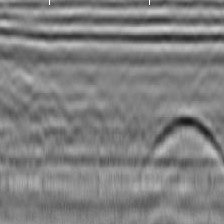
\includegraphics[width=0.45\linewidth]{example-011.jpg}}
  \hfill
  \subfloat[Annotated single-target sample.]{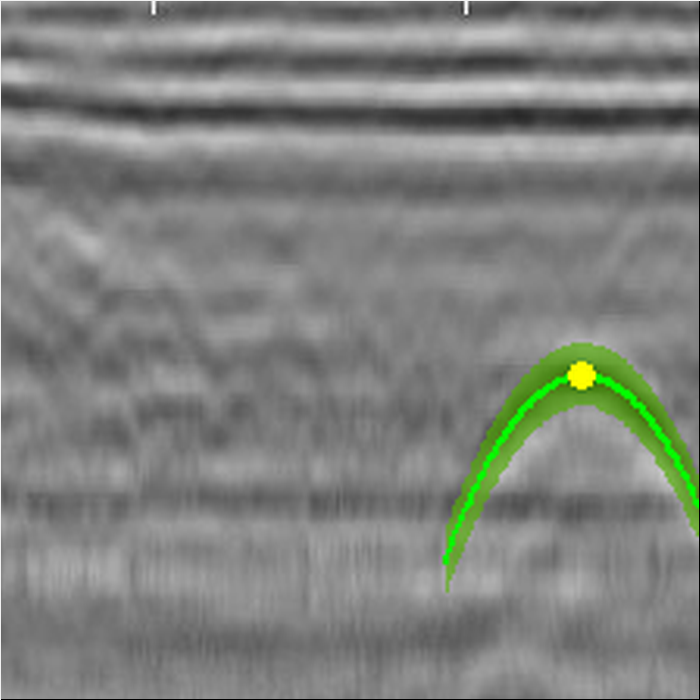
\includegraphics[width=0.45\linewidth]{example-011-labelled.png}}\\
  \subfloat[Raw multi-target sample.]{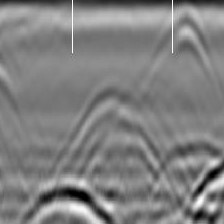
\includegraphics[width=0.45\linewidth]{example-030.jpg}}
  \hfill
  \subfloat[Annotated multi-target sample.]{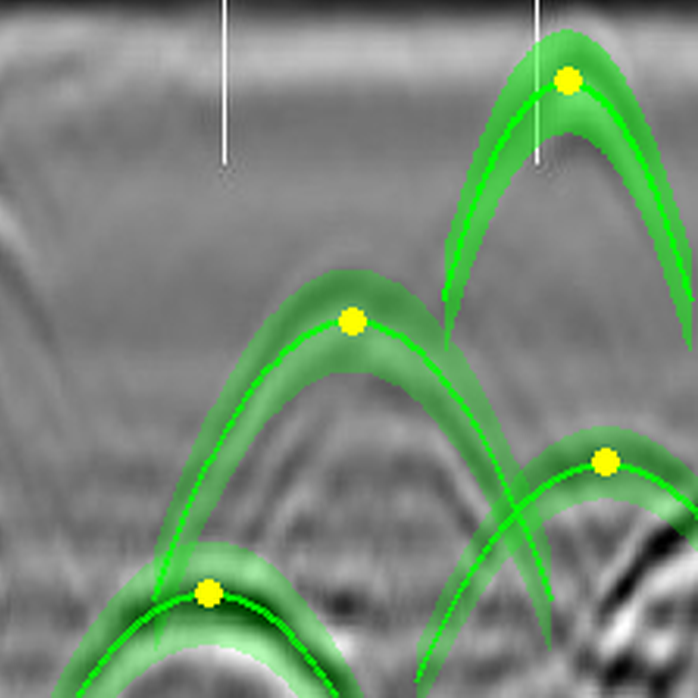
\includegraphics[width=0.45\linewidth]{example-030-labelled.png}}
  \caption{Examples of hyperbola samples and their labeled visualizations.}
  \label{fig:dataset_samples}
\end{figure}

\subsection{Result1}

\begin{table*}[]
\centering
\caption{Detection performance (mean $\pm$ std over 10 seeds) at different
training-data fractions. ``abs'' uses the attention constraint with
$\lambda_{\mathrm{att}}=0.7$.}
\label{tab:bbox_results}
\setlength{\tabcolsep}{4pt}
\renewcommand{\arraystretch}{1.2}
\begin{tabular}{c ccc ccc}
\toprule
\multirow{2}{*}{\textbf{Frac.}} &
\multicolumn{3}{c}{\textbf{none}} &
\multicolumn{3}{c}{\textbf{abs} ($\lambda{=}0.7$)} \\
\cmidrule(lr){2-4} \cmidrule(lr){5-7}
 & \textbf{P} & \textbf{R} & \textbf{F1}
 & \textbf{P} & \textbf{R} & \textbf{F1} \\
\midrule
0.5 & 0.811\,$\pm$\,0.200 & 0.425\,$\pm$\,0.094 & 0.529\,$\pm$\,0.075
    & 0.855\,$\pm$\,0.082 & 0.487\,$\pm$\,0.070 & \textbf{0.617\,$\pm$\,0.063} \\
0.6 & 0.711\,$\pm$\,0.213 & 0.560\,$\pm$\,0.083 & 0.600\,$\pm$\,0.098
    & 0.754\,$\pm$\,0.254 & 0.645\,$\pm$\,0.064 & \textbf{0.663\,$\pm$\,0.131} \\
0.7 & 0.752\,$\pm$\,0.304 & 0.679\,$\pm$\,0.097 & 0.678\,$\pm$\,0.207
    & 0.905\,$\pm$\,0.079 & 0.782\,$\pm$\,0.046 & \textbf{0.836\,$\pm$\,0.032} \\
0.8 & 0.843\,$\pm$\,0.223 & 0.821\,$\pm$\,0.071 & 0.811\,$\pm$\,0.159
    & 0.909\,$\pm$\,0.122 & 0.882\,$\pm$\,0.041 & \textbf{0.890\,$\pm$\,0.069} \\
0.9 & 0.875\,$\pm$\,0.238 & 0.900\,$\pm$\,0.068 & 0.867\,$\pm$\,0.172
    & 0.847\,$\pm$\,0.223 & 0.931\,$\pm$\,0.044 & \textbf{0.870\,$\pm$\,0.165} \\
\bottomrule
\end{tabular}
\end{table*}

%加上可视化的比较 他漏掉了什么 我们对了什么
\subsection{Result2}
%和其他注意力机制比较  ok
\begin{table}[htbp]
\centering
\begin{tabular}{lccc}
\hline
config & bbox\_P & bbox\_R & bbox\_F1 \\
\hline
None    & 0.843\,$\pm$\,0.223 & 0.821\,$\pm$\,0.071 & 0.811\,$\pm$\,0.159 \\
se       & $0.8559\pm0.1948$ & $0.8164\pm0.0417$ & $0.8205\pm0.1123$ \\
cbam     & $0.7478\pm0.1649$ & $0.8186\pm0.0290$ & $0.7709\pm0.0966$ \\
nonlocal & $0.8438\pm0.2818$ & $0.7361\pm0.2245$ & $0.7825\pm0.2510$ \\
coord    & $0.8017\pm0.2339$ & $0.8355\pm0.0904$ & $0.7979\pm0.1722$ \\
Ours     & 0.909\,$\pm$\,0.122 & 0.882\,$\pm$\,0.041 & \textbf{0.890\,$\pm$\,0.069} \\
\hline
\end{tabular}
\caption{Comparison of detection performance with different attention modules}
\label{tab:attention_comparison}
\end{table}
\subsection{Result3}
%在其他的识别框架中也有效 和centernet框架比较嘛

\subsection{Result4}
%放在其他的预训练的backbone中也有效 ok

\subsection{Result3}
%看一下heatmap的图 证明注意力真的有效

\subsection{Result3}
%参数敏感性分析 lam 从0.1开始嘛 ok



\subsection{Result3}
%软性的约束是不是可能会更加好 如果lam参数调节好的话
\section{Discussion}



\section*{Acknowledgments}
This should be a simple paragraph before the References to thank those individuals and institutions who have supported your work on this article.



{\appendix[Proof of the Zonklar Equations]
Use $\backslash${\tt{appendix}} if you have a single appendix:
Do not use $\backslash${\tt{section}} anymore after $\backslash${\tt{appendix}}, only $\backslash${\tt{section*}}.
If you have multiple appendixes use $\backslash${\tt{appendices}} then use $\backslash${\tt{section}} to start each appendix.
You must declare a $\backslash${\tt{section}} before using any $\backslash${\tt{subsection}} or using $\backslash${\tt{label}} ($\backslash${\tt{appendices}} by itself
 starts a section numbered zero.)}



%{\appendices
%\section*{Proof of the First Zonklar Equation}
%Appendix one text goes here.
% You can choose not to have a title for an appendix if you want by leaving the argument blank
%\section*{Proof of the Second Zonklar Equation}
%Appendix two text goes here.}



\bibliographystyle{IEEEtran}
\bibliography{1references}


\newpage

\section{Biography Section}
If you have an EPS/PDF photo (graphicx package needed), extra braces are
 needed around the contents of the optional argument to biography to prevent
 the LaTeX parser from getting confused when it sees the complicated
 $\backslash${\tt{includegraphics}} command within an optional argument. (You can create
 your own custom macro containing the $\backslash${\tt{includegraphics}} command to make things
 simpler here.)
 
\vspace{11pt}

\bf{If you include a photo:}\vspace{-33pt}
\begin{IEEEbiography}[{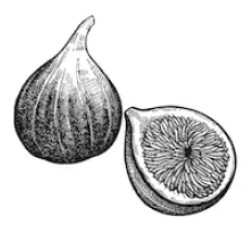
\includegraphics[width=1in,height=1.25in,clip,keepaspectratio]{fig1}}]{Michael Shell}
Use $\backslash${\tt{begin\{IEEEbiography\}}} and then for the 1st argument use $\backslash${\tt{includegraphics}} to declare and link the author photo.
Use the author name as the 3rd argument followed by the biography text.
\end{IEEEbiography}

\vspace{11pt}

\bf{If you will not include a photo:}\vspace{-33pt}
\begin{IEEEbiographynophoto}{John Doe}
Use $\backslash${\tt{begin\{IEEEbiographynophoto\}}} and the author name as the argument followed by the biography text.
\end{IEEEbiographynophoto}




\vfill

\end{document}


